% Options for packages loaded elsewhere
\PassOptionsToPackage{unicode}{hyperref}
\PassOptionsToPackage{hyphens}{url}
%
\documentclass[
]{article}
\usepackage{amsmath,amssymb}
\usepackage{lmodern}
\usepackage{ifxetex,ifluatex}
\ifnum 0\ifxetex 1\fi\ifluatex 1\fi=0 % if pdftex
  \usepackage[T1]{fontenc}
  \usepackage[utf8]{inputenc}
  \usepackage{textcomp} % provide euro and other symbols
\else % if luatex or xetex
  \usepackage{unicode-math}
  \defaultfontfeatures{Scale=MatchLowercase}
  \defaultfontfeatures[\rmfamily]{Ligatures=TeX,Scale=1}
  \setmainfont[]{serif}
\fi
% Use upquote if available, for straight quotes in verbatim environments
\IfFileExists{upquote.sty}{\usepackage{upquote}}{}
\IfFileExists{microtype.sty}{% use microtype if available
  \usepackage[]{microtype}
  \UseMicrotypeSet[protrusion]{basicmath} % disable protrusion for tt fonts
}{}
\makeatletter
\@ifundefined{KOMAClassName}{% if non-KOMA class
  \IfFileExists{parskip.sty}{%
    \usepackage{parskip}
  }{% else
    \setlength{\parindent}{0pt}
    \setlength{\parskip}{6pt plus 2pt minus 1pt}}
}{% if KOMA class
  \KOMAoptions{parskip=half}}
\makeatother
\usepackage{xcolor}
\IfFileExists{xurl.sty}{\usepackage{xurl}}{} % add URL line breaks if available
\IfFileExists{bookmark.sty}{\usepackage{bookmark}}{\usepackage{hyperref}}
\hypersetup{
  pdftitle={Leveraging Machine Learning to Study How Temperament Scores Predict Pre-Term Birth Status.},
  pdfauthor={Jennifer Mattera, Erich Seamon, XXX, Maria A. Gartstein},
  hidelinks,
  pdfcreator={LaTeX via pandoc}}
\urlstyle{same} % disable monospaced font for URLs
\usepackage[margin=1in]{geometry}
\usepackage{graphicx}
\makeatletter
\def\maxwidth{\ifdim\Gin@nat@width>\linewidth\linewidth\else\Gin@nat@width\fi}
\def\maxheight{\ifdim\Gin@nat@height>\textheight\textheight\else\Gin@nat@height\fi}
\makeatother
% Scale images if necessary, so that they will not overflow the page
% margins by default, and it is still possible to overwrite the defaults
% using explicit options in \includegraphics[width, height, ...]{}
\setkeys{Gin}{width=\maxwidth,height=\maxheight,keepaspectratio}
% Set default figure placement to htbp
\makeatletter
\def\fps@figure{htbp}
\makeatother
\setlength{\emergencystretch}{3em} % prevent overfull lines
\providecommand{\tightlist}{%
  \setlength{\itemsep}{0pt}\setlength{\parskip}{0pt}}
\setcounter{secnumdepth}{-\maxdimen} % remove section numbering
\usepackage{pdflscape}
\newcommand{\blandscape}{\begin{landscape}}
\newcommand{\elandscape}{\end{landscape}}
\usepackage{setspace}\doublespacing
\renewcommand{\figurename}{Figure S}
\renewcommand{\tablename}{Table S}
\usepackage{booktabs}
\usepackage{longtable}
\usepackage{array}
\usepackage{multirow}
\usepackage{wrapfig}
\usepackage{float}
\usepackage{colortbl}
\usepackage{pdflscape}
\usepackage{tabu}
\usepackage{threeparttable}
\usepackage{threeparttablex}
\usepackage[normalem]{ulem}
\usepackage{makecell}
\usepackage{xcolor}
\ifluatex
  \usepackage{selnolig}  % disable illegal ligatures
\fi

\title{Leveraging Machine Learning to Study How Temperament Scores
Predict Pre-Term Birth Status.}
\usepackage{etoolbox}
\makeatletter
\providecommand{\subtitle}[1]{% add subtitle to \maketitle
  \apptocmd{\@title}{\par {\large #1 \par}}{}{}
}
\makeatother
\subtitle{The material contained herein is supplementary to the article
named in the title and submitted to the journal, XXX.}
\author{Jennifer Mattera, Erich Seamon, XXX, Maria A. Gartstein}
\date{10/25/2022}

\begin{document}
\maketitle

This supplemental appendix provides machine learning analyses figures
and tables in support of the following paper: "", submitted to XXXX.

\newpage

\listoffigures
\listoftables
\newpage

\newpage

\begin{figure}[H]

{\centering 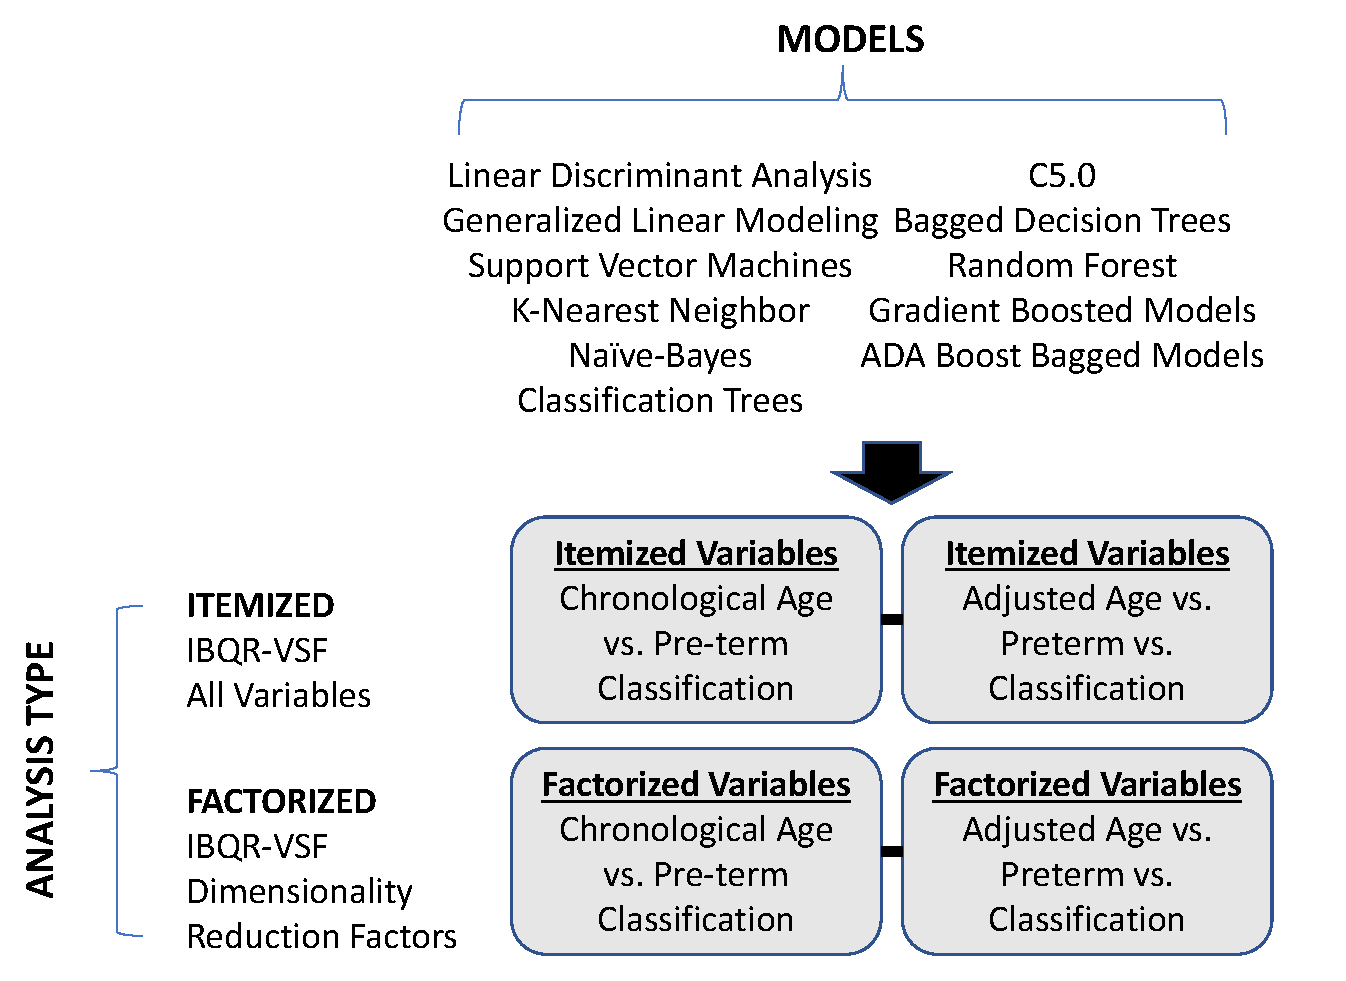
\includegraphics[width=0.75\linewidth]{./images/Figure1} 

}

\caption{Quantitative methodology:  Four analysis types were considered. For each analysis type, 11 classification machine learning algorithms were used, resulting in a total of 44 model outputs.}\label{fig:image-ref-for-in-text}
\end{figure}
\newpage

\hypertarget{section}{%
\section{}\label{section}}

\pagebreak
\begin{table}

\caption{\label{tab:unnamed-chunk-3}Infant Behavior Questionnaire-Revised Very Short Form Items - Surgency}
\fontsize{12}{14}\selectfont
\begin{tabular}[t]{>{\raggedright\arraybackslash}p{40em}}
\hline
\textbf{Surgency}\\
\hline
Item 1: When being dressed or undressed during the last week, how often did the baby squirm and/or try to roll away?\\
\hline
Item 2: When tossed around playfully how often did the baby laugh?\\
\hline
Item 7: How often during the week did your baby move quickly toward new objects?\\
\hline
Item 8: When put into the bath water, how often did the baby laugh?\\
\hline
Item 13: When placed on his/her back, how often did the baby squirm and/or turn body?\\
\hline
Item 14: During a peekaboo game, how often did the baby laugh?\\
\hline
Item 15: How often does the infant look up from playing when the telephone rings?\\
\hline
Item 20: When visiting a new place, how often did your baby get excited about exploring new surroundings?\\
\hline
Item 21: How often during the last week did the baby smile or laugh when given a toy?\\
\hline
Item 26: When hair was washed, how often did the baby vocalize?\\
\hline
Item 27: How often did your baby notice the sound of an airplane passing overhead?\\
\hline
Item 36: How often did your baby make talking sounds when riding in a car?\\
\hline
Item 37: When placed in an infant seat or car seat, how often did the baby squirm and turn body?\\
\hline
\end{tabular}
\end{table}

\hypertarget{section-1}{%
\section{}\label{section-1}}

\pagebreak

\begin{table}

\caption{\label{tab:unnamed-chunk-4}Infant Behavior Questionnaire-Revised Very Short Form Items - Negative Affect}
\fontsize{12}{14}\selectfont
\begin{tabular}[t]{>{\raggedright\arraybackslash}p{40em}}
\hline
\textbf{Negative Affect}\\
\hline
Item 3: When tired, how often did your baby show distress?\\
\hline
Item 4: When introduced to an unfamiliar adult, how often did the baby cling to a parent?\\
\hline
Item 9: When it was time for bed or a nap and your baby did not want to go, how often did s/he whimper or sob?\\
\hline
Item 10: After sleeping, how often did the baby cry if someone doesn’t come within a few minutes?\\
\hline
Item 16: How often did the baby seem angry (crying and fussing) when you left her/him in the crib?\\
\hline
Item 17: How often during the last week did the baby startle at a sudden change in body position (e.g., when moved suddenly)?\\
\hline
Item 22: At the end of an exciting day, how often did your baby become tearful?\\
\hline
Item 23: How often during the last week did the baby protest being placed in a confining place (infant seat, play pen, car seat, etc.)?\\
\hline
Item 28: When introduced to an unfamiliar adult, how often did the baby refuse to go to the unfamiliar person?\\
\hline
Item 29: When you were busy with another activity, and your baby was not able to get your attention, how often did s/he cry?\\
\hline
Item 32: When the baby wanted something, how often did s/he become upset when s/he could not get what s/he wanted?\\
\hline
Item 33: When in the presence of several unfamiliar adults, how often did the baby cling to a parent?\\
\hline
\end{tabular}
\end{table}

\hypertarget{section-2}{%
\section{}\label{section-2}}

\pagebreak
\begin{table}

\caption{\label{tab:unnamed-chunk-5}Infant Behavior Questionnaire-Revised Very Short Form Items - Effortful Control}
\fontsize{12}{14}\selectfont
\begin{tabular}[t]{>{\raggedright\arraybackslash}p{40em}}
\hline
\textbf{Effortful Control}\\
\hline
Item 5: How often during the last week did the baby enjoy being read to?\\
\hline
Item 6: How often during the last week did the baby play with one toy or object for 5-10 minutes?\\
\hline
Item 11: In the last week, while being fed in your lap, how often did the baby seem eager to get away as soon as the feeding was over?\\
\hline
Item 12: When singing or talking to your baby, how often did s/he soothe immediately?\\
\hline
Item 18: How often during the last week did the baby enjoy hearing the sound of words, as in nursery rhymes?\\
\hline
Item 19: How often during the last week did the baby look at pictures in books and/or magazines for 5 minutes or longer at a time?\\
\hline
Item 24: When being held, in the last week, did your baby seem to enjoy him/herself?\\
\hline
Item 25: When showing the baby something to look at, how often did s/he soothe immediately?\\
\hline
Item 30: How often during the last week did the baby enjoy gentle rhythmic activities, such as rocking or swaying?\\
\hline
Item 31: How often during the last week did the baby stare at a mobile, crib bumper or picture for 5 minutes or longer?\\
\hline
Item 34: When rocked or hugged, in the last week, did your baby seem to enjoy him/herself?\\
\hline
Item 35: When patting or gently rubbing some part of the baby’s body, how often did s/he soothe immediately?\\
\hline
\end{tabular}
\end{table}

\newpage

\begin{figure}

{\centering 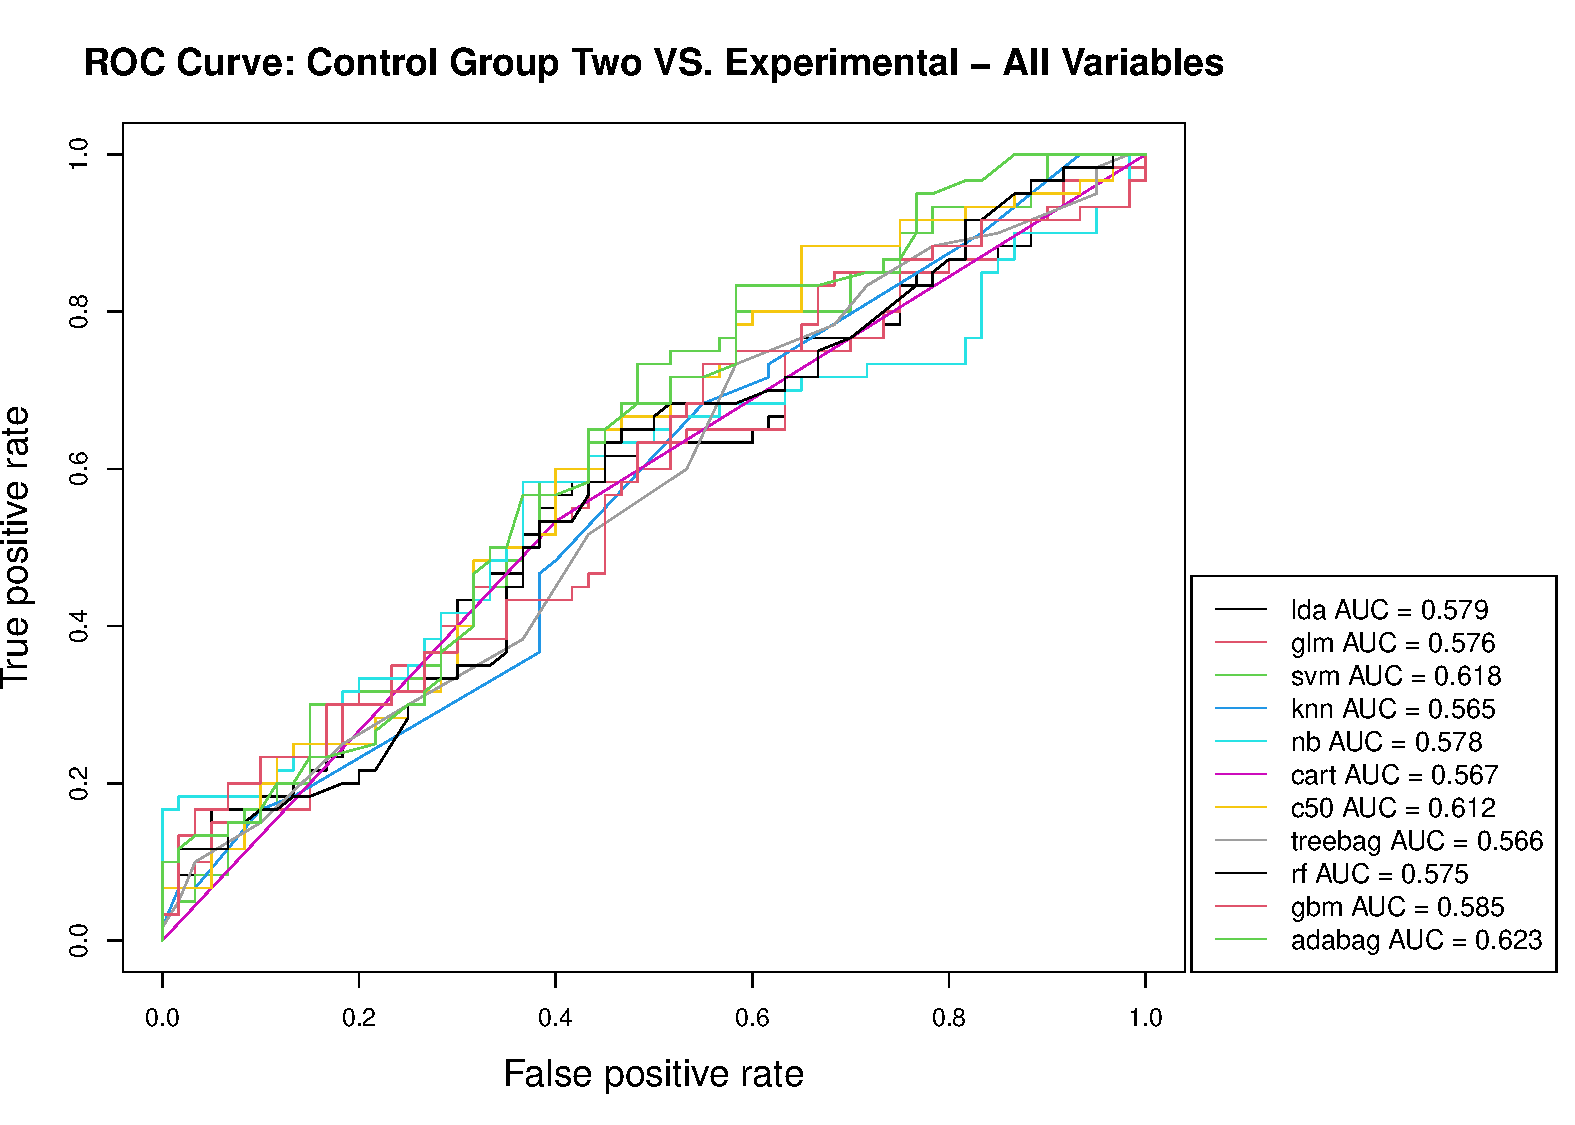
\includegraphics{Supplemental_Materials_files/figure-latex/unnamed-chunk-6-1} 

}

\caption{Accuracy Estimates: Chronological Age Group vs. Pre-Term Group - Itemized Variables.}\label{fig:unnamed-chunk-6}
\end{figure}
\newpage

\begin{figure}

{\centering 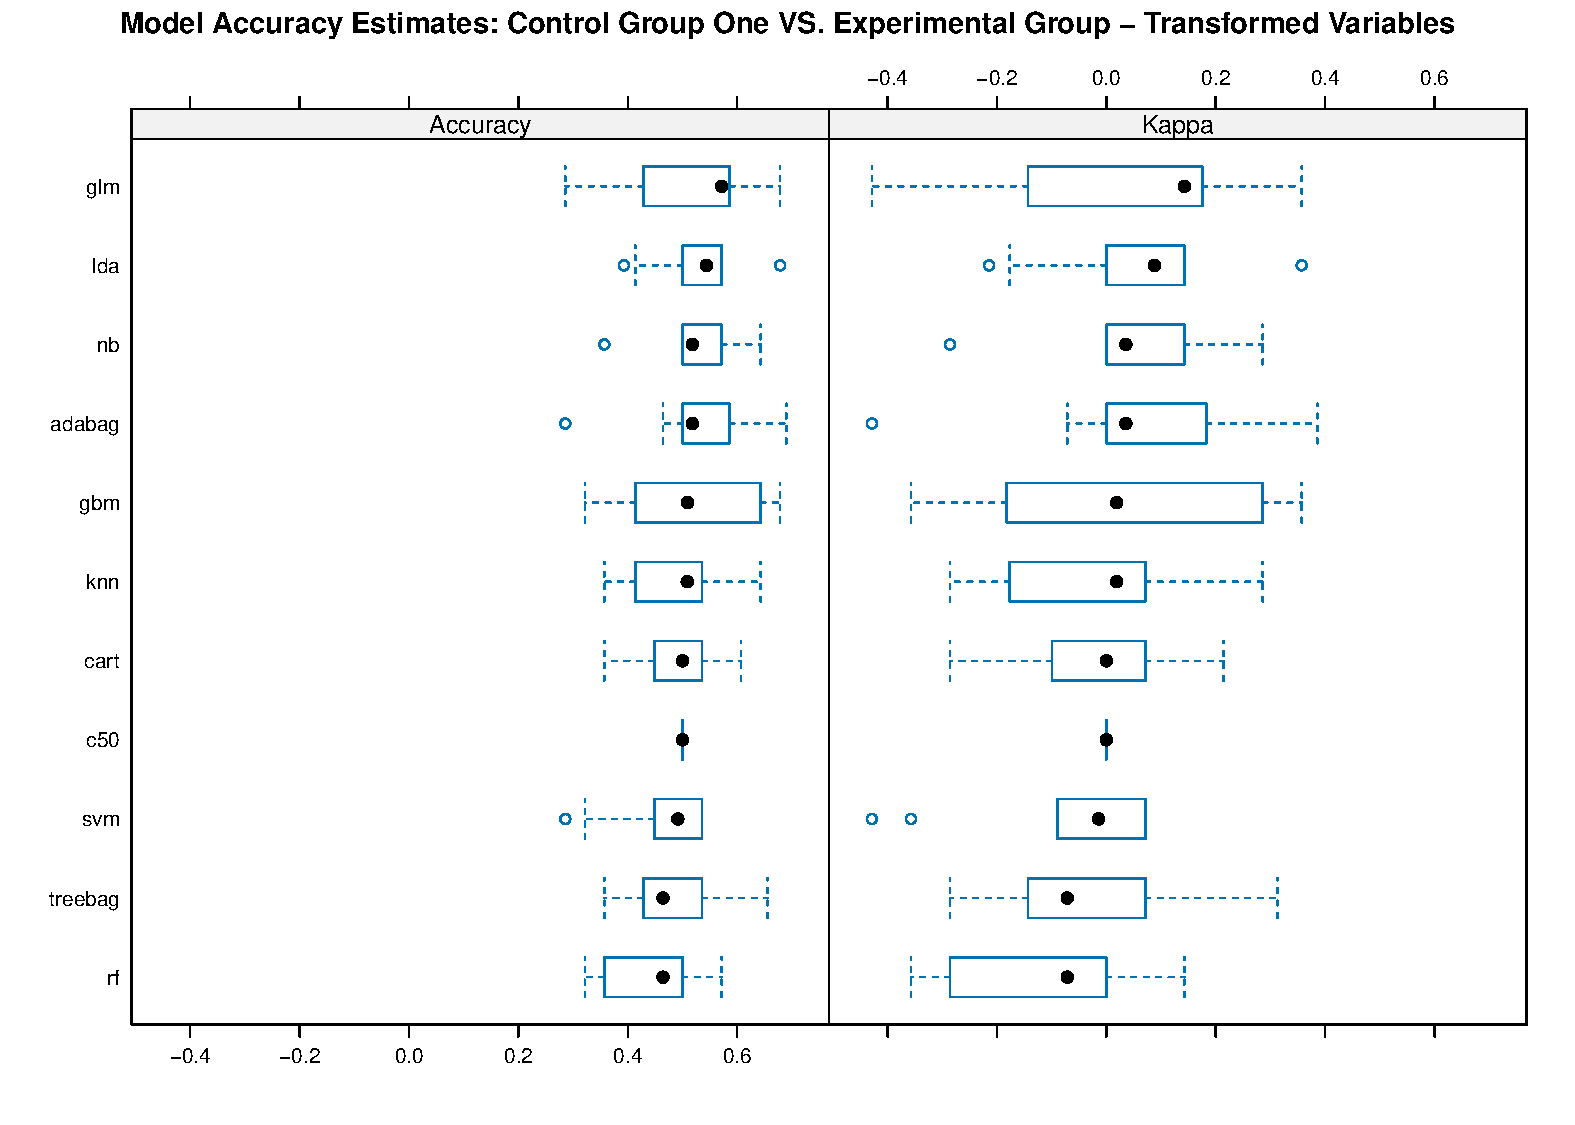
\includegraphics{Supplemental_Materials_files/figure-latex/unnamed-chunk-7-1} 

}

\caption{Receiver Operator Curve: Chronological Age Group vs. Pre-Term Group - Itemized Variables.}\label{fig:unnamed-chunk-7}
\end{figure}

\newpage

\begin{figure}

{\centering 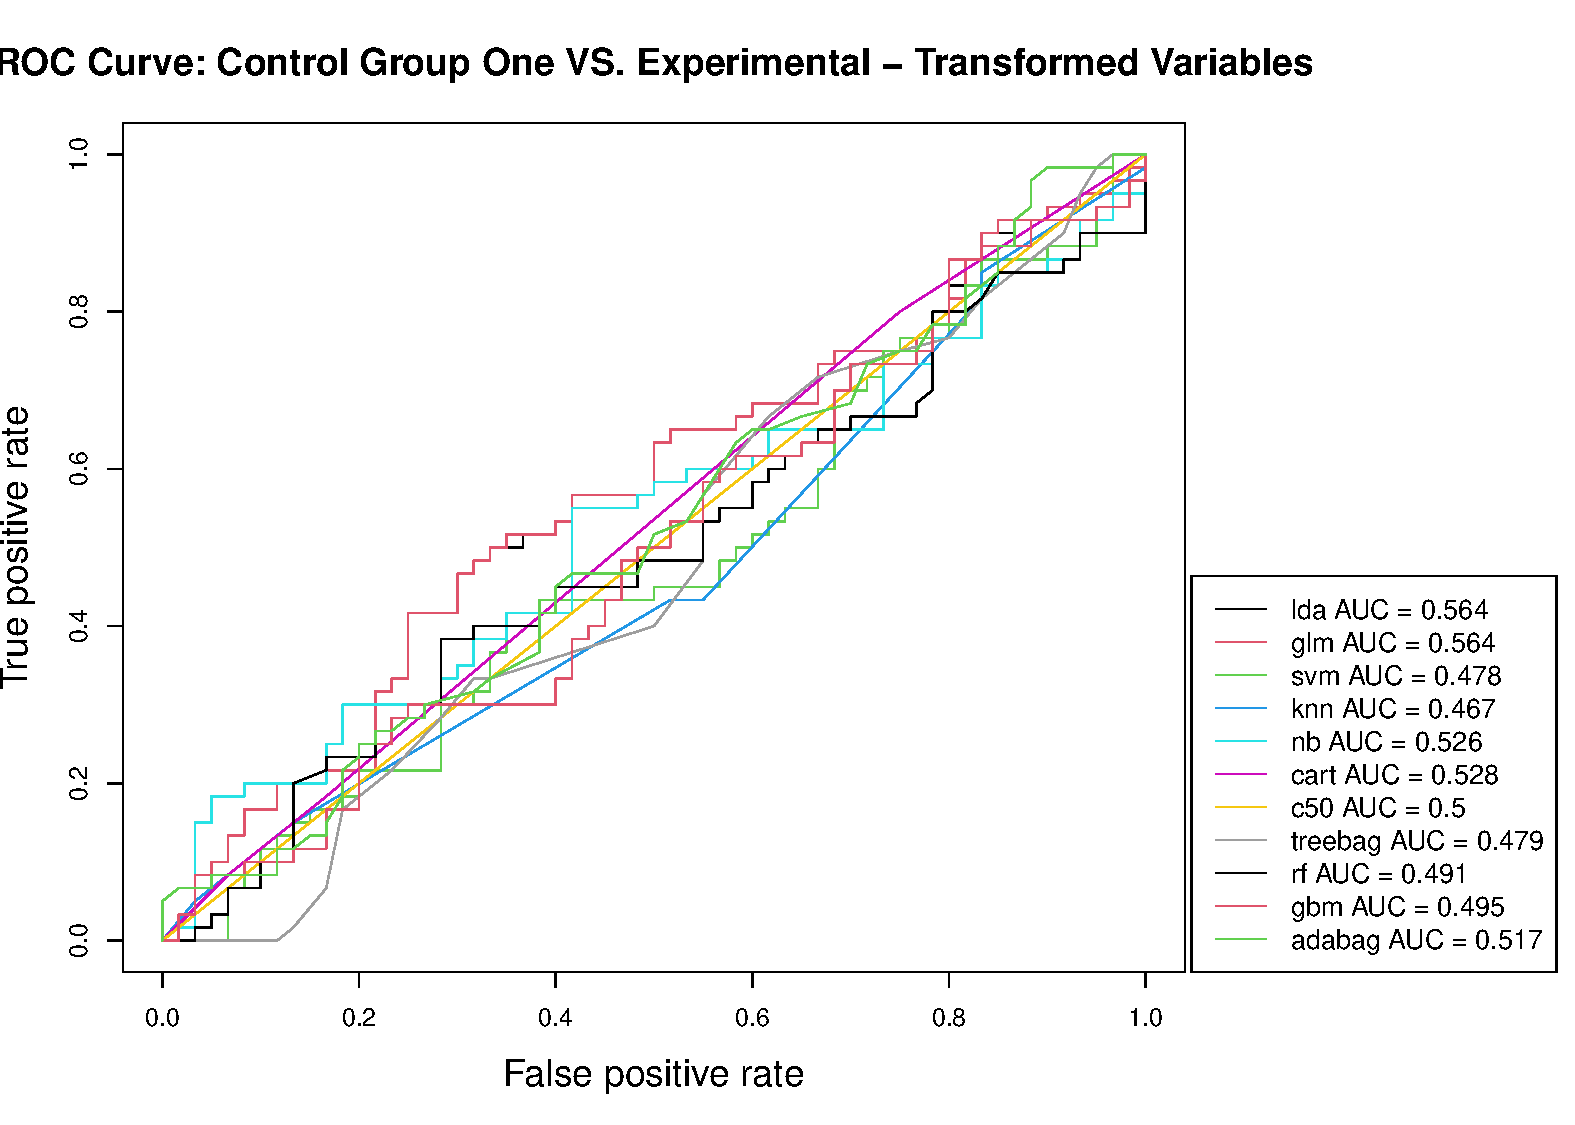
\includegraphics{Supplemental_Materials_files/figure-latex/unnamed-chunk-8-1} 

}

\caption{Accuracy Estimates: Age Adjusted Group vs. Pre-Term Group - Itemized Variables.}\label{fig:unnamed-chunk-8}
\end{figure}
\newpage

\begin{figure}

{\centering 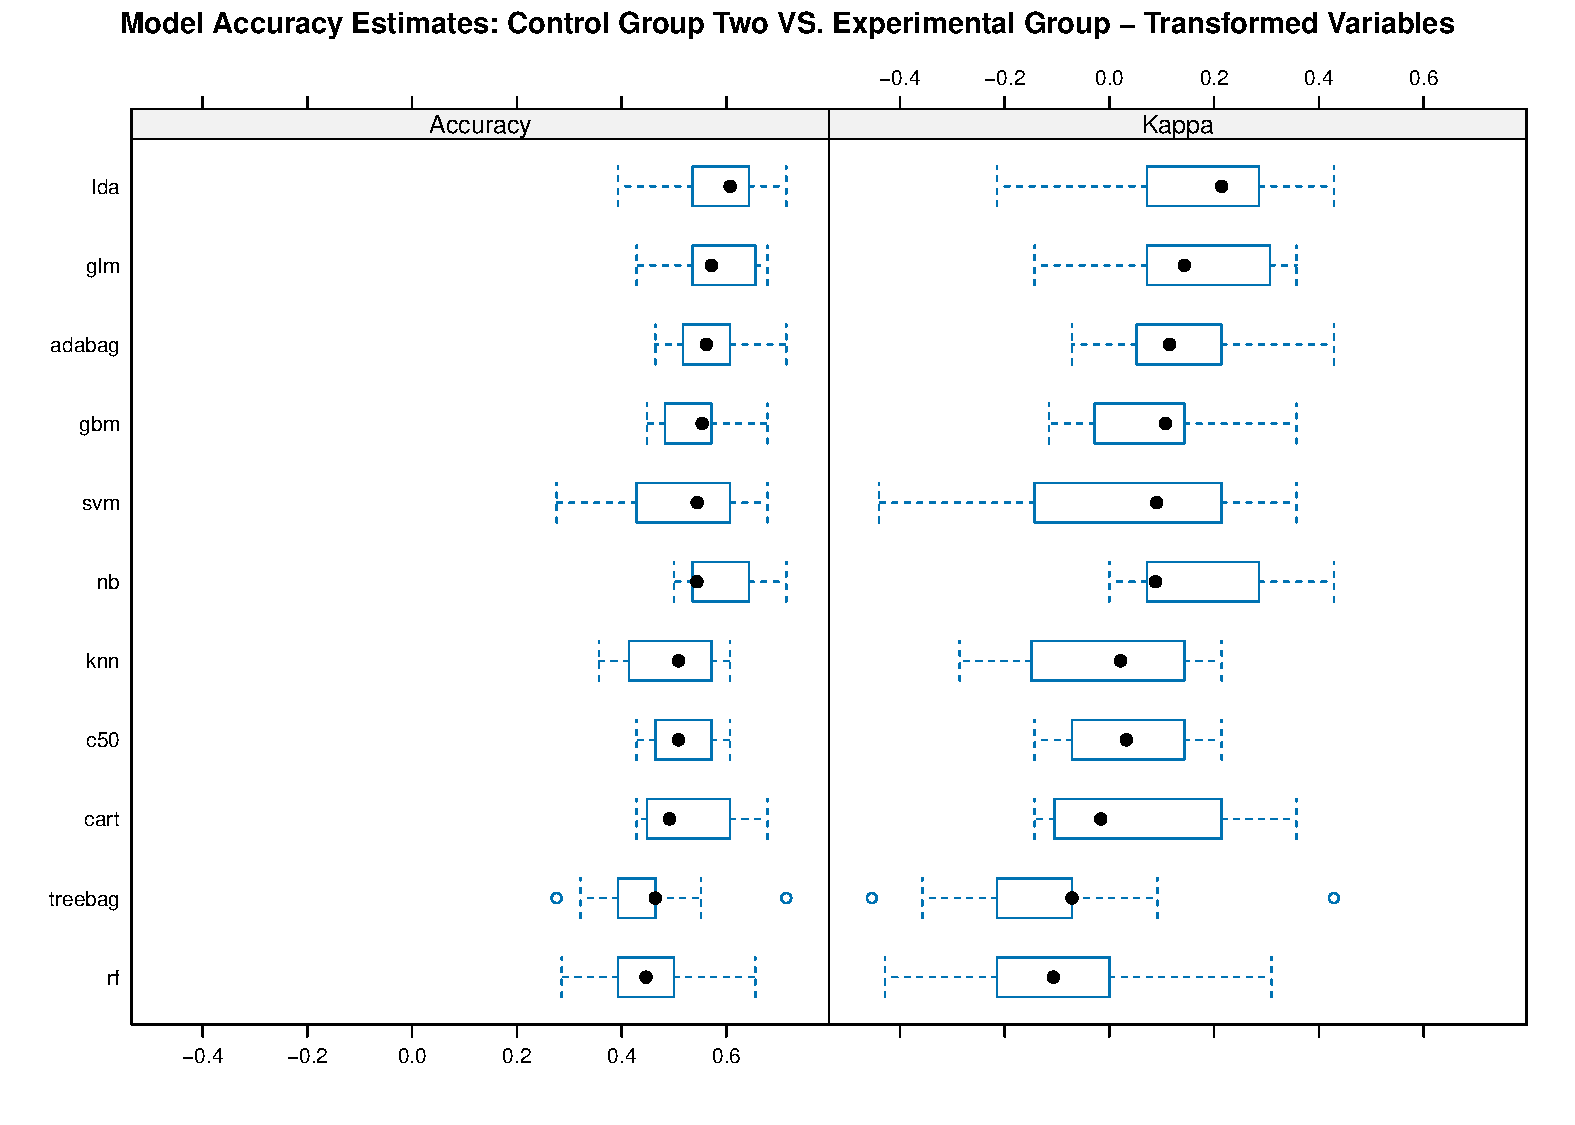
\includegraphics{Supplemental_Materials_files/figure-latex/unnamed-chunk-9-1} 

}

\caption{Receiver Operator Curve: Age Adjusted Group vs. Pre-Term Group - Itemized Variables.}\label{fig:unnamed-chunk-9}
\end{figure}

\newpage

\begin{figure}

{\centering 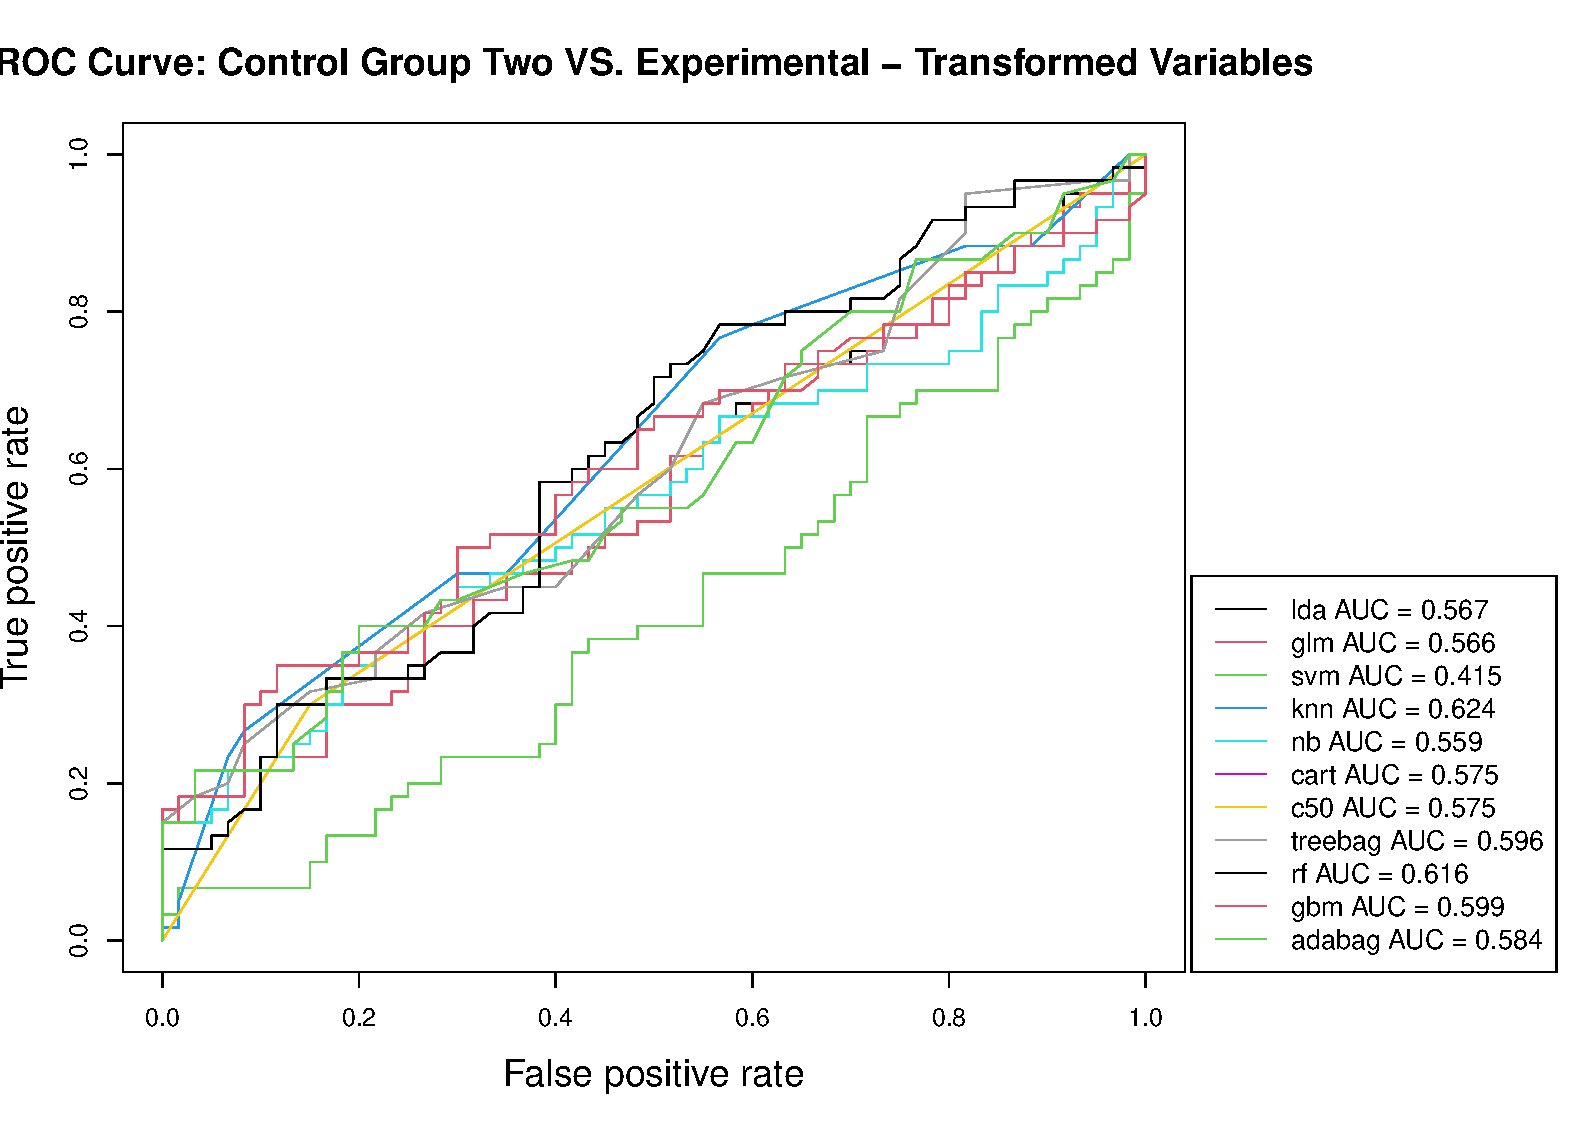
\includegraphics{Supplemental_Materials_files/figure-latex/unnamed-chunk-10-1} 

}

\caption{Accuracy Estimates: Chronological Age Group vs. Pre-Term Group - Factorized Variables.}\label{fig:unnamed-chunk-10}
\end{figure}

\newpage

\begin{figure}

{\centering \includegraphics{Supplemental_Materials_files/figure-latex/unnamed-chunk-11-1} 

}

\caption{Receiver Operator Curve: Chronological Age Group vs. Pre-Term Group - Factorized Variables.}\label{fig:unnamed-chunk-11}
\end{figure}
\newpage

\begin{figure}

{\centering 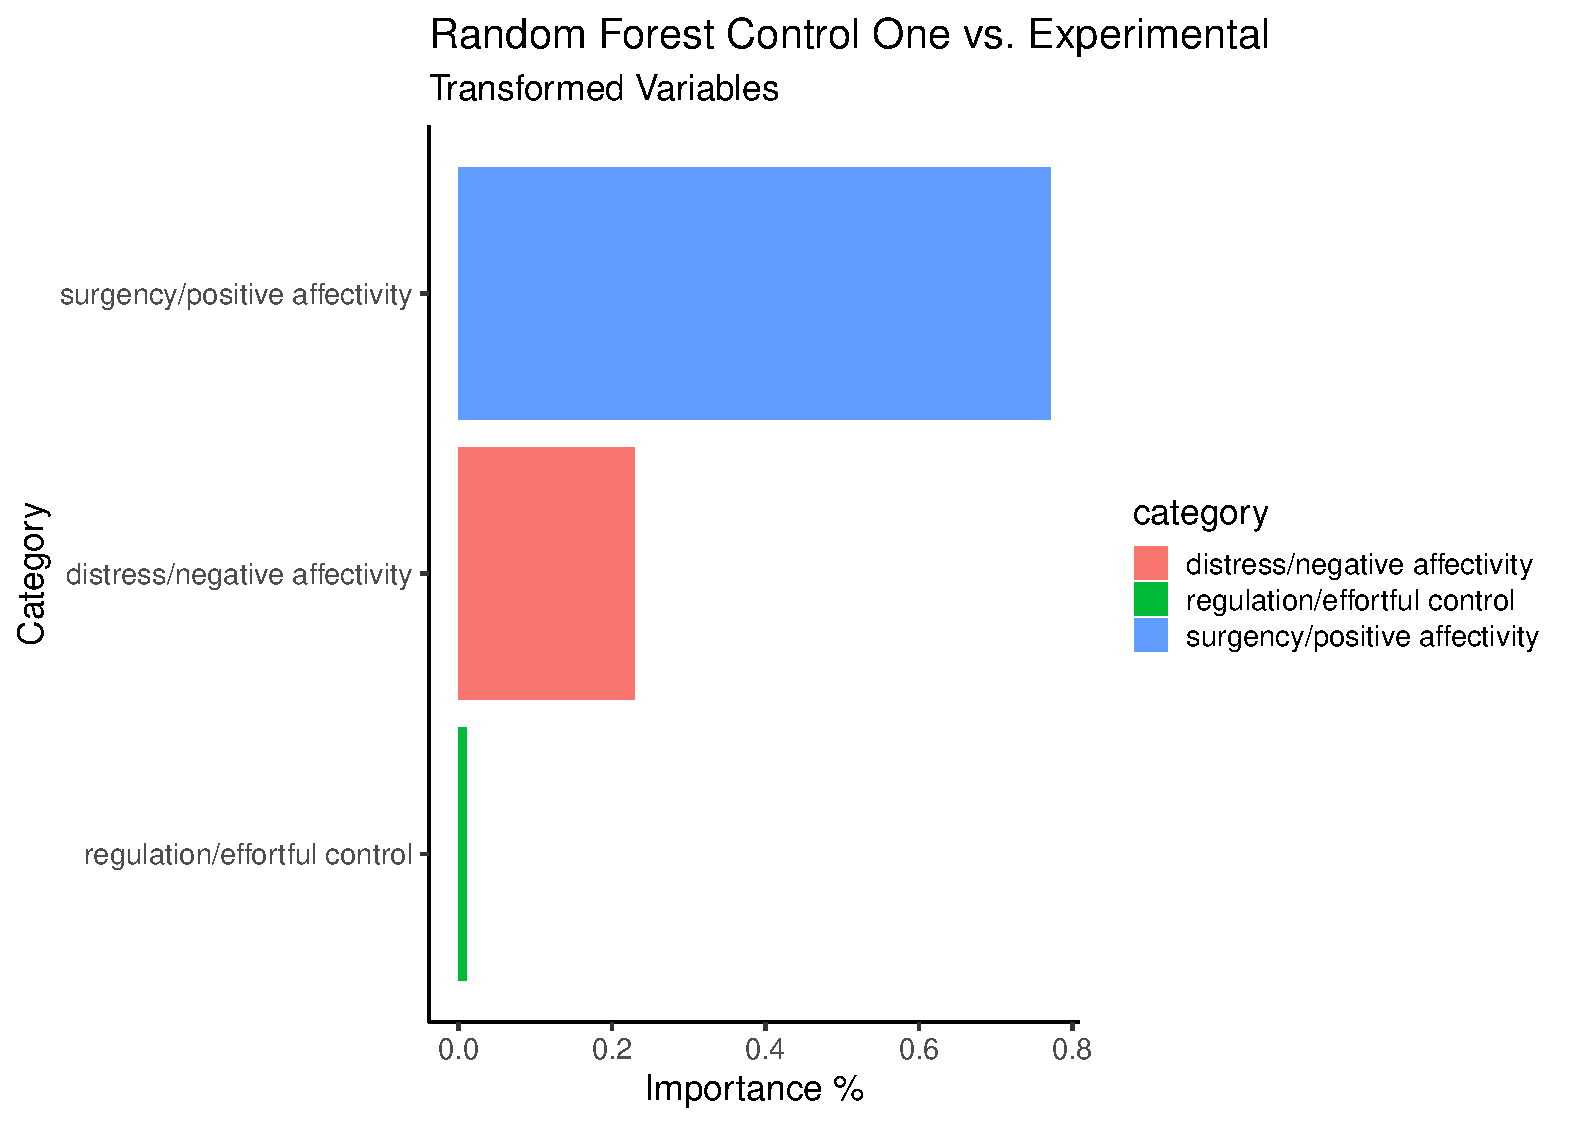
\includegraphics{Supplemental_Materials_files/figure-latex/unnamed-chunk-12-1} 

}

\caption{Accuracy Estimates: Age Adjusted Group vs. Pre-Term Group - Factorized Variables.}\label{fig:unnamed-chunk-12}
\end{figure}

\newpage

\begin{figure}

{\centering 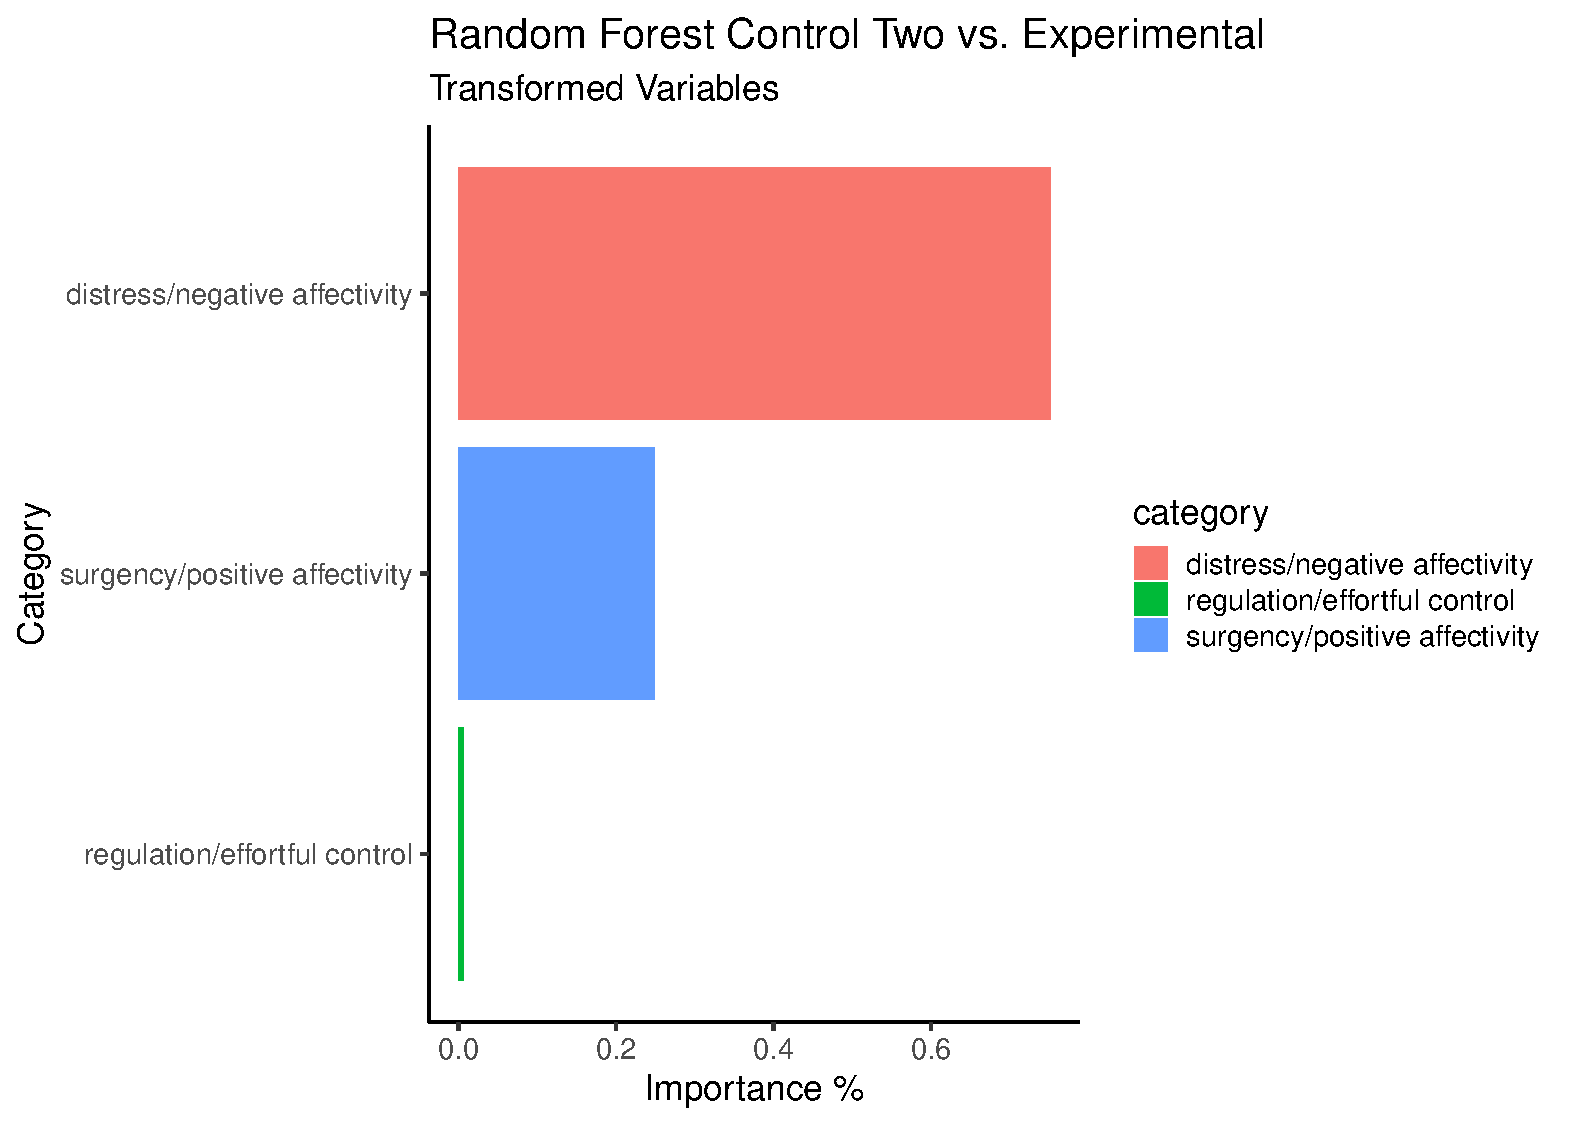
\includegraphics{Supplemental_Materials_files/figure-latex/unnamed-chunk-13-1} 

}

\caption{Receiver Operator Curve: Age Adjusted Group vs. Pre-Term Group - Factorized Variables.}\label{fig:unnamed-chunk-13}
\end{figure}
\newpage

\begin{figure}

{\centering 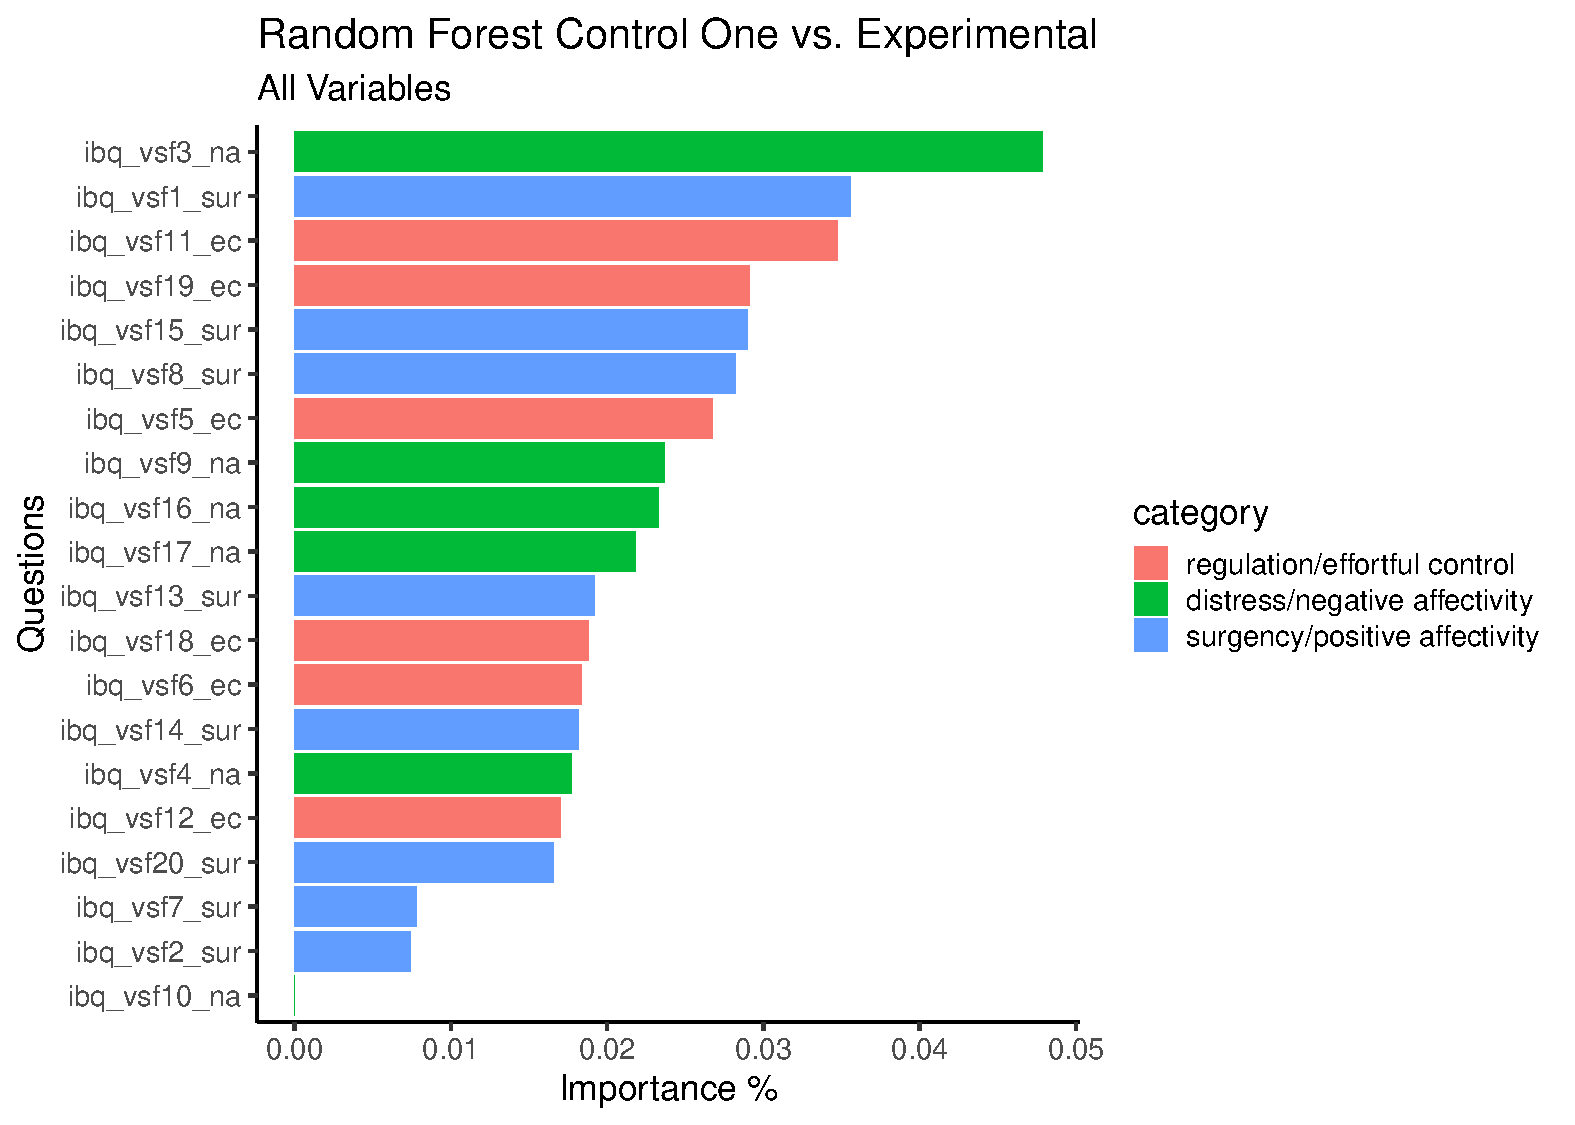
\includegraphics{Supplemental_Materials_files/figure-latex/unnamed-chunk-15-1} 

}

\caption{Feature Importance: Chronological Age Group vs. Pre-Term Group - Factorized Variables}\label{fig:unnamed-chunk-15}
\end{figure}

\newpage

\begin{figure}

{\centering 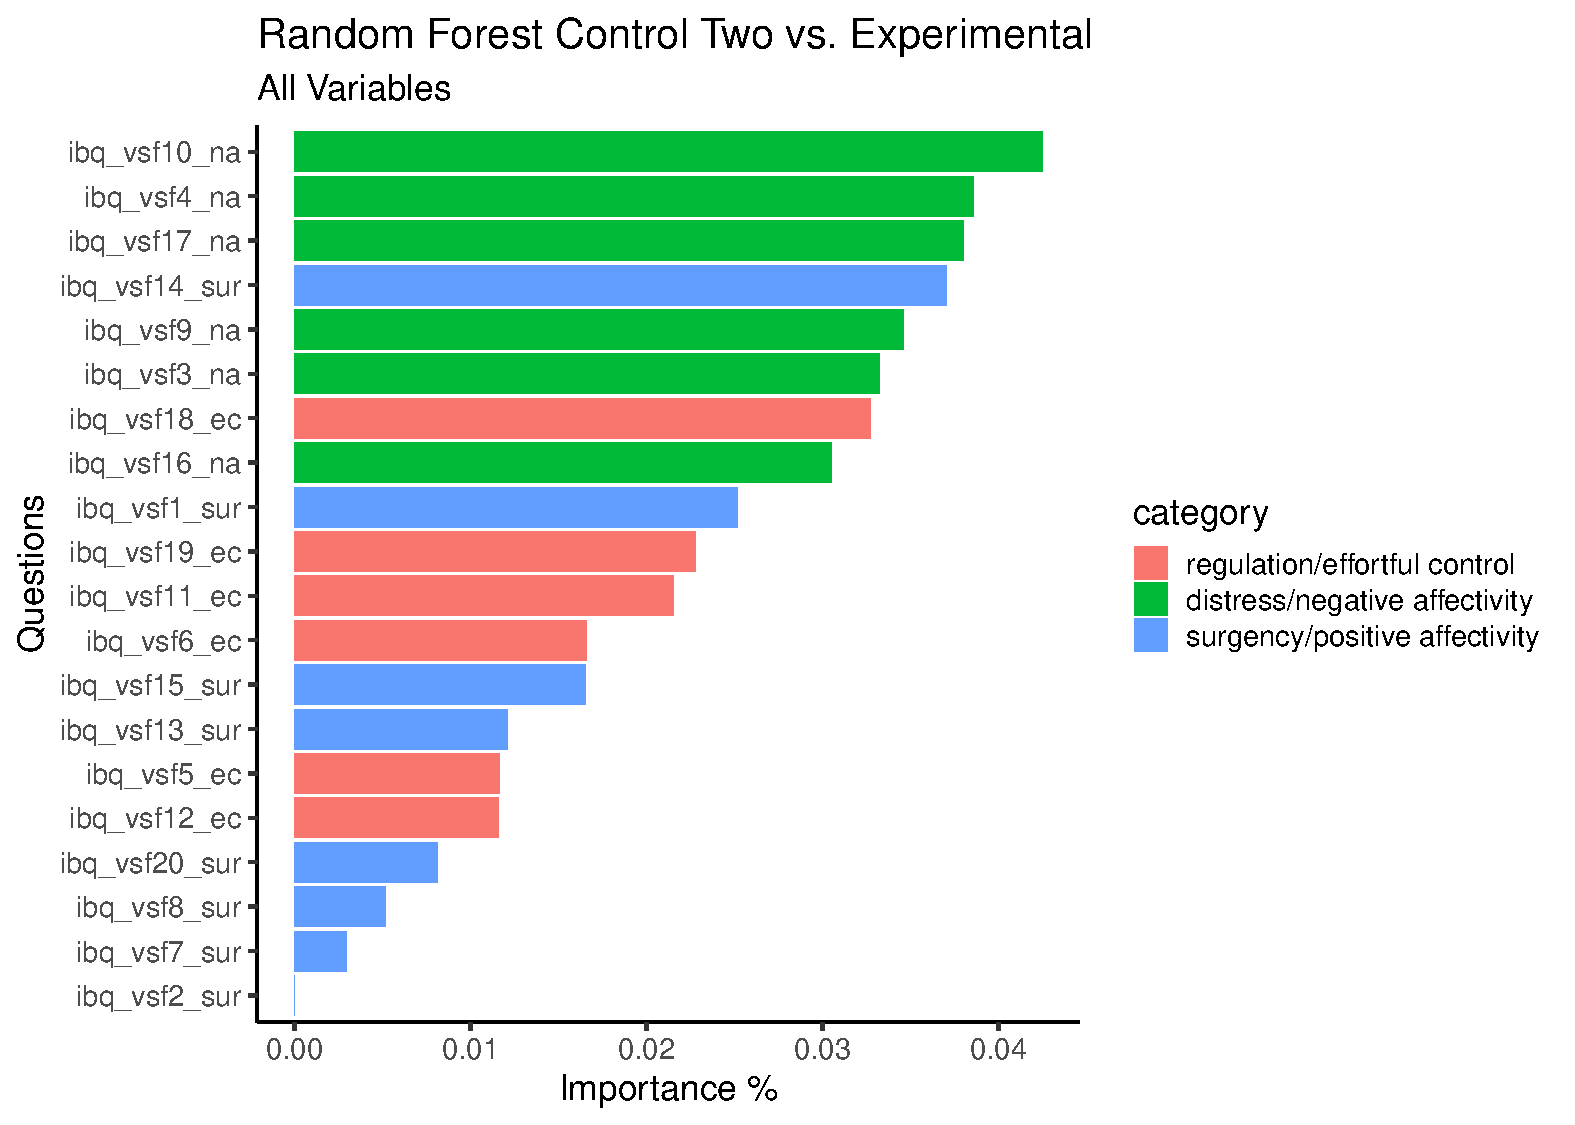
\includegraphics{Supplemental_Materials_files/figure-latex/unnamed-chunk-16-1} 

}

\caption{Feature Importance: Age Adjusted Group vs. Pre-Term Group - Factorized Variables}\label{fig:unnamed-chunk-16}
\end{figure}
\newpage

\newpage

\begin{figure}

{\centering \includegraphics{Supplemental_Materials_files/figure-latex/unnamed-chunk-18-1} 

}

\caption{Feature Importance: Chronological Age Group vs. Pre-Term Group - Itemized Variables}\label{fig:unnamed-chunk-18}
\end{figure}

\newpage

\begin{figure}

{\centering \includegraphics{Supplemental_Materials_files/figure-latex/unnamed-chunk-19-1} 

}

\caption{Feature Importance: Age Adjusted Group vs. Pre-Term Group - Itemized Variables}\label{fig:unnamed-chunk-19}
\end{figure}

\newpage

\begin{table}

\caption{\label{tab:unnamed-chunk-21}Model Results: Itemized Variables}
\fontsize{12}{14}\selectfont
\begin{tabular}[t]{l|r|r|r|r|r|r}
\hline
\multicolumn{1}{c|}{models} & \multicolumn{3}{c|}{Chronological VS. Pre-Term: Itemized} & \multicolumn{3}{c}{Adjusted Age VS. Pre-Term: Itemized} \\
\cline{1-1} \cline{2-4} \cline{5-7}
  & accuracy & kappa & AUC & accuracy & kappa & AUC\\
\hline
lda & 0.493 & -0.014 & 0.617 & 0.504 & 0.009 & 0.579\\
\hline
glm & 0.490 & -0.021 & 0.621 & 0.524 & 0.047 & 0.576\\
\hline
svm & 0.493 & -0.016 & 0.550 & 0.557 & 0.113 & 0.618\\
\hline
knn & 0.581 & 0.162 & 0.603 & 0.542 & 0.085 & 0.565\\
\hline
nb & 0.542 & 0.084 & 0.576 & 0.579 & 0.156 & 0.578\\
\hline
cart & 0.539 & 0.078 & 0.542 & 0.490 & -0.020 & 0.567\\
\hline
c5.0 & 0.475 & -0.051 & 0.615 & 0.514 & 0.029 & 0.566\\
\hline
bagging & 0.517 & 0.032 & 0.617 & 0.532 & 0.063 & 0.575\\
\hline
rf & 0.500 & 0.001 & 0.646 & 0.574 & 0.149 & 0.585\\
\hline
gbm & 0.503 & 0.008 & 0.600 & 0.582 & 0.163 & 0.623\\
\hline
adabag & 0.543 & 0.084 & 0.617 & 0.546 & 0.093 & 0.579\\
\hline
\end{tabular}
\end{table}

\newpage

\begin{table}

\caption{\label{tab:unnamed-chunk-22}Model Results: Factorized Variables}
\fontsize{12}{14}\selectfont
\begin{tabular}[t]{l|r|r|r|r|r|r}
\hline
\multicolumn{1}{c|}{models} & \multicolumn{3}{c|}{Chronological VS. Pre-Term: Factorized} & \multicolumn{3}{c}{Adjusted Age VS. Pre-Term: Factorized} \\
\cline{1-1} \cline{2-4} \cline{5-7}
  & accuracy & kappa & AUC & accuracy & kappa & AUC\\
\hline
lda & 0.532 & 0.064 & 0.564 & 0.581 & 0.162 & 0.567\\
\hline
glm & 0.525 & 0.050 & 0.564 & 0.585 & 0.169 & 0.566\\
\hline
svm & 0.457 & -0.083 & 0.478 & 0.519 & 0.038 & 0.415\\
\hline
knn & 0.458 & -0.086 & 0.467 & 0.497 & -0.004 & 0.624\\
\hline
nb & 0.525 & 0.050 & 0.526 & 0.578 & 0.156 & 0.559\\
\hline
cart & 0.493 & -0.014 & 0.528 & 0.504 & 0.008 & 0.575\\
\hline
c5.0 & 0.497 & -0.007 & 0.479 & 0.514 & 0.029 & 0.596\\
\hline
bagging & 0.485 & -0.029 & 0.491 & 0.454 & -0.093 & 0.616\\
\hline
rf & 0.447 & -0.105 & 0.495 & 0.449 & -0.102 & 0.599\\
\hline
gbm & 0.489 & -0.022 & 0.517 & 0.547 & 0.093 & 0.584\\
\hline
adabag & 0.492 & -0.014 & 0.564 & 0.568 & 0.135 & 0.567\\
\hline
\end{tabular}
\end{table}

\newpage

\begin{figure}

{\centering \includegraphics{Supplemental_Materials_files/figure-latex/unnamed-chunk-24-1} 

}

\caption{R2 Comparisons - Chronological Age Group VS Pre-Term Group, Factorized Variables VS. Itemized Variables.}\label{fig:unnamed-chunk-24}
\end{figure}

\begin{figure}

{\centering \includegraphics{Supplemental_Materials_files/figure-latex/unnamed-chunk-25-1} 

}

\caption{AUC Comparisons - Chronological Age Group VS Pre-Term Group, Factorized Variables VS. Itemized Variables.}\label{fig:unnamed-chunk-25}
\end{figure}

\begin{figure}

{\centering \includegraphics{Supplemental_Materials_files/figure-latex/unnamed-chunk-26-1} 

}

\caption{R2 Comparisons - Age Adjusted Group VS Pre-Term Group, Factorized Variables VS. Itemized Variables.}\label{fig:unnamed-chunk-26}
\end{figure}

\begin{figure}

{\centering \includegraphics{Supplemental_Materials_files/figure-latex/unnamed-chunk-27-1} 

}

\caption{AUC Comparisons - Age Adjusted Group VS Pre-Term Group, Factorized Variables VS. Itemized Variables.}\label{fig:unnamed-chunk-27}
\end{figure}

\end{document}
